\documentclass[12pt]{article}
\usepackage{verbatim}
\usepackage[dvips]{epsfig}
\usepackage{color}
\usepackage{url}
\usepackage[colorlinks=true]{hyperref}

\begin{document}

\section*{GENESIS: Documentation}

{\bf Related Documentation:}
% start: userdocs-tag-replace-items related-do-nothing
% end: userdocs-tag-replace-items related-do-nothing

\section*{Installing from a Debian Package}

Debian packages will be available for all major components of GENESIS via Sourceforge at:
\begin{itemize}
   \item[]\href{https://sourceforge.net/projects/genesis-sim/}{https://sourceforge.net/projects/genesis-sim/}
\end{itemize}
\noindent or
\begin{itemize}
   \item[]\href{http://genesis-sim.org/downloads}{http://genesis-sim.org/downloads}
\end{itemize}
This allows for easy installation via the Debian Package installer GUI.

{\bf Note:} If your computer is not correctly configured for GENESIS (i.e. the correct \href{../genesis-dependencies/genesis-dependencies.tex}{software dependencies} are not installed in the expected locations) the Debian Package installer will issue a warning and request that the missing package be installed.

\subsection*{Installation via Package Installer}

Simply download the desired package to your machine. Go to the directory where it was downloaded. This directory should have an appropriate `package' icon.

\begin{figure}[h]
   \centering
   
\includegraphics[scale=1]{figures/install-user-deb-icon.eps}
%   \label{fig:df-1}
\end{figure}

Double click on the package icon. A form will appear that gives details about the package such as: Package description, Dependencies, and files to be installed.

\begin{figure}[h]
   \centering
   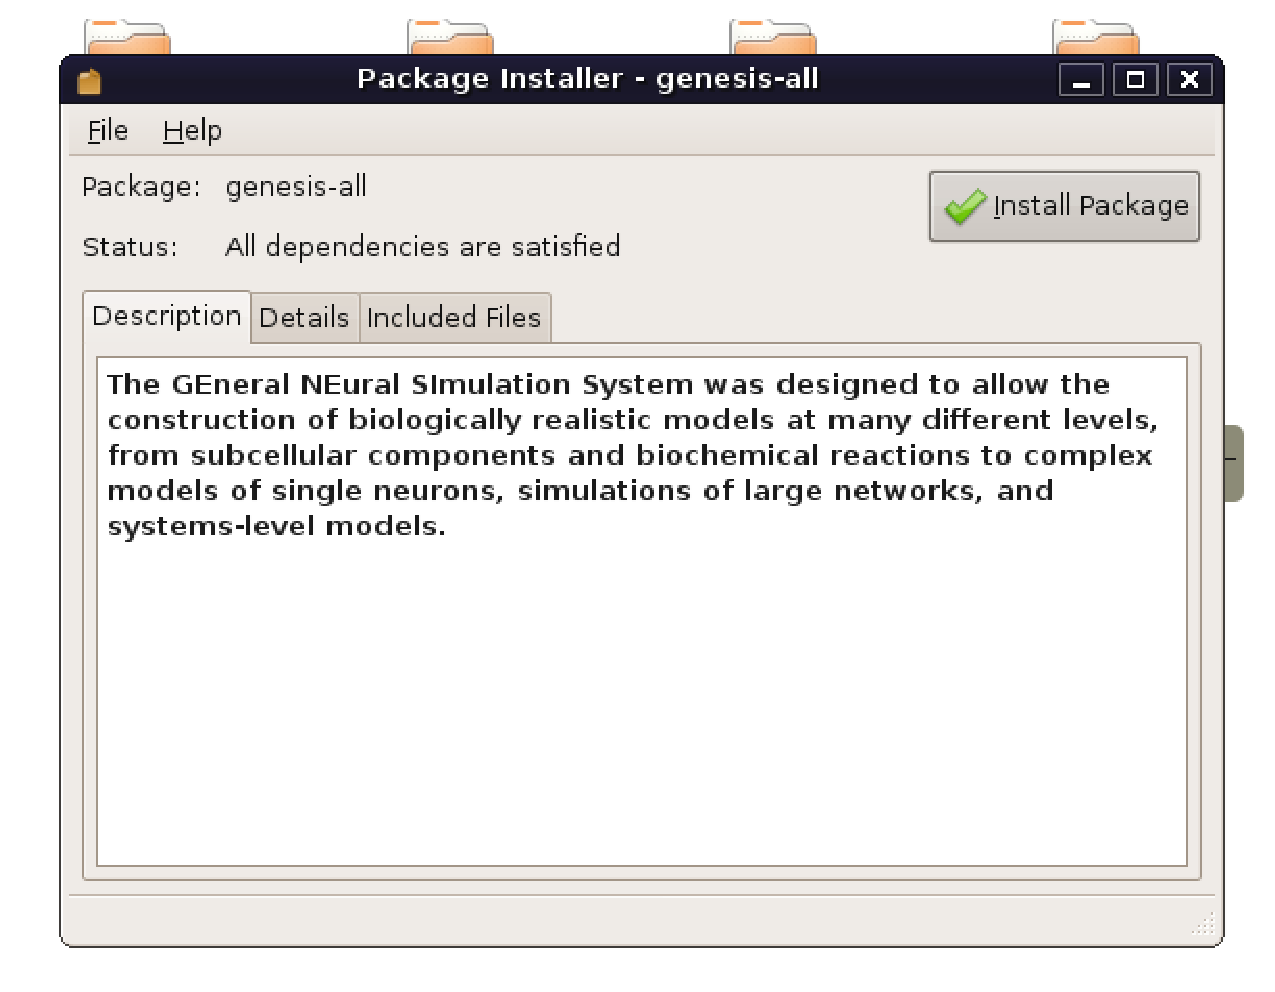
\includegraphics[scale=0.5]{figures/install-user-deb-pkg.eps}
%   \label{fig:df-1}
\end{figure}

\newpage

Click on the ``{\sf Install Package}'' button and you will be prompted to enter the administrator password to proceed with the installation.

\begin{figure}[h]
   \centering
   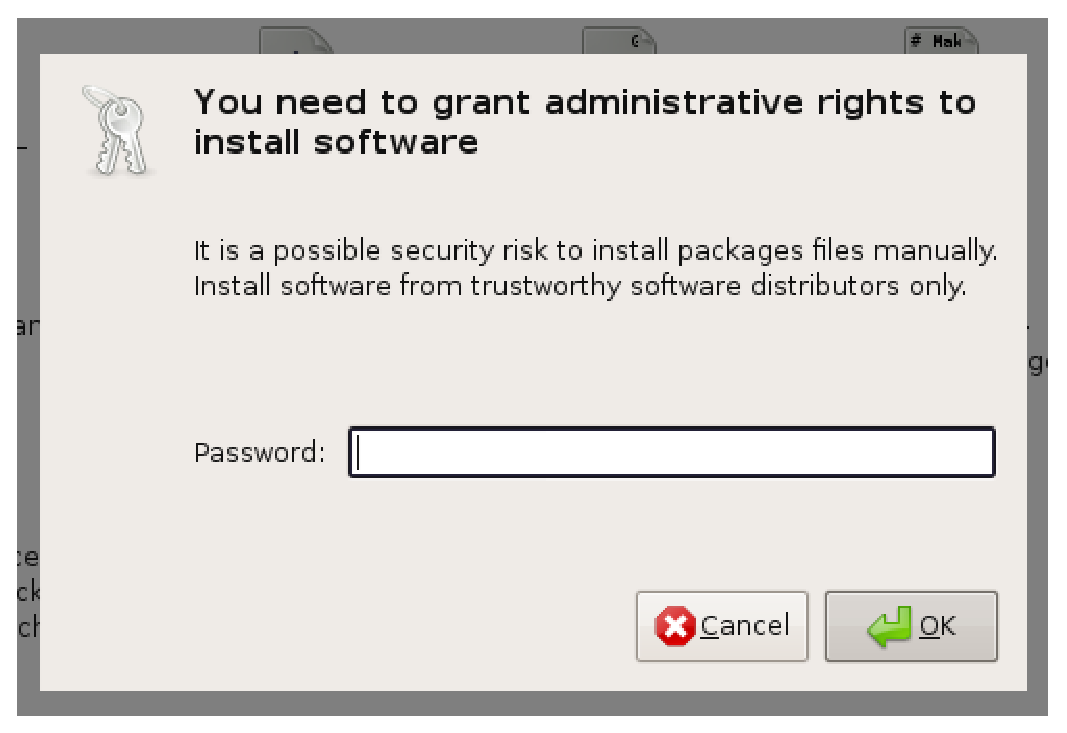
\includegraphics[scale=0.5]{figures/install-user-deb-admin.eps}
%   \label{fig:df-1}
\end{figure}

Once the installation is complete the package installer will prompt with a `{\sf Finished}' message.

\subsection*{Removing a Debian Package via the Command Line}

A Debian package can be removed from the system via the command:
\begin{verbatim}
   sudo apt-get --purge remove <package-name>
\end{verbatim}
where {\tt <package-name>} is replaced with the name of the {\bf .deb} package that was previously installed. 

\end{document}
